%
% qclsip: The Quantum Cascade Laser Stock Image Project.
%
% Copyright (c) 2019, Computational Photonics Group, Technical University of
% Munich.
%
% Simple QCL geometry.
% Created by Michael Riesch <michael.riesch@tum.de> (2019)
%
% This program is free software; you can redistribute it and/or modify
% it under the terms of the GNU General Public License as published by
% the Free Software Foundation; either version 3 of the License, or
% (at your option) any later version.
%
% This program is distributed in the hope that it will be useful,
% but WITHOUT ANY WARRANTY; without even the implied warranty of
% MERCHANTABILITY or FITNESS FOR A PARTICULAR PURPOSE.  See the
% GNU General Public License for more details.
%
% You should have received a copy of the GNU General Public License
% along with this program; if not, write to the Free Software Foundation,
% Inc., 51 Franklin Street, Fifth Floor, Boston, MA 02110-1301  USA
\documentclass[tikz]{standalone}

\usepackage[utf8]{inputenc}
\usepackage[T1]{fontenc}
\usepackage{tikz}

% set colors
\usepackage{xcolor}
\definecolor{sipblue}{RGB}{0,101,189} % Pantone 300
\definecolor{sipdarkblue}{RGB}{0,82,147} % Pantone 301
\definecolor{siplightblue}{RGB}{152,198,234} % Pantone 283
\definecolor{sipmedblue}{RGB}{100,160,200} % Pantone 542
\definecolor{sipivory}{RGB}{218,215,203} % Pantone 7527
\definecolor{sipgreen}{RGB}{162,173,0} % Pantone 383
\definecolor{siporange}{RGB}{227,114,34} % Pantone 158
\definecolor{sipgray}{gray}{0.6} % Gray 60%

% set font
\usepackage{helvet}
\renewcommand{\familydefault}{\sfdefault}

\begin{document}
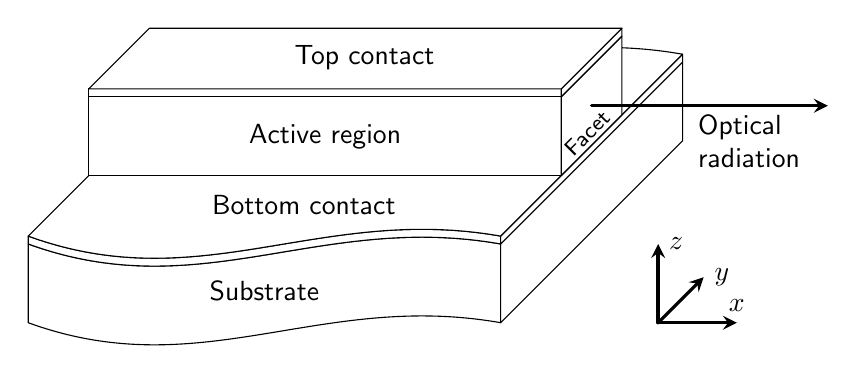
\begin{tikzpicture}
  \tikzstyle{myline}=[black, line cap=round,line join=round];
  %
  % coordinate system
  \tikzstyle{cs}=[myline, very thick, ->, >=stealth];
  \begin{scope}[shift={(8, 0, 6)}]
    \draw[cs] (0, 0, 0) -- (1, 0, 0) node[above] {$x$};
    \draw[cs] (0, 0, 0) -- (0, 1, 0) node[right] {$z$};
    \draw[cs] (0, 0, 0) -- (0, 0, -1.5) node[right] {$y$};
  \end{scope}
  %
  % substrate
  \tikzstyle{sub}=[myline, fill=white];
  \coordinate (subA) at (0, 0, 6);
  \coordinate (subB) at (6, 0, 6);
  \coordinate (subC) at (6, 1, 6);
  \coordinate (subD) at (0, 1, 6);
  \coordinate (subE) at (6, 0, 0);
  \coordinate (subF) at (6, 1, 0);
  % the curved path gives a large bounding box -> ignore with overlay
  \draw[sub, overlay] (subA) to[out=-20, in=170] (subB)
  -- (subC) to[out=170, in=-20] (subD) -- (subA);
  % dummy point that fixes  bounding box
  \node[] at (1, 0, 6.5) {};
  \draw[sub] (subB) -- (subE) -- (subF) -- (subC) -- (subB);
  \node[] at (3, 0.4, 6) {Substrate};
  %
  % bottom contact
  \tikzstyle{bot}=[myline, fill=white];
  \begin{scope}[shift={(0, 1, 0)}]
    \coordinate (botA) at (0, 0, 6);
    \coordinate (botB) at (6, 0, 6);
    \coordinate (botC) at (6, 0.1, 6);
    \coordinate (botD) at (0, 0.1, 6);
    \coordinate (botE) at (6, 0, 0);
    \coordinate (botF) at (6, 0.1, 0);
    \coordinate (botG) at (0, 0.1, 0);
    \draw[bot] (botA) to[out=-20, in=170] (botB) -- (botC)
    to[out=170, in=-20] (botD) -- (botA);
    \draw[bot] (botB) -- (botE) -- (botF) -- (botC) -- (botB);
    % the curved path gives a large bounding box -> ignore with overlay
    \draw[bot, overlay] (botD) to[out=-20, in=170] (botC) -- (botF)
    to[out=170, in=-20] (botG) -- (botD);
    \node[] at (3, 0, 4.7) {Bottom contact};
  \end{scope}
  %
  % active region
  \tikzstyle{act}=[myline, fill=white];
  \begin{scope}[shift={(0, 1.1, 0)}]
    \coordinate (actA) at (0, 0, 4);
    \coordinate (actB) at (6, 0, 4);
    \coordinate (actC) at (6, 1, 4);
    \coordinate (actD) at (0, 1, 4);
    \coordinate (actE) at (6, 0, 2);
    \coordinate (actF) at (6, 1, 2);
    \draw[act] (actA) -- (actB) -- (actC) -- (actD) -- (actA);
    % facet part
    \draw[act] (actB) -- (actE) -- (actF) -- (actC) -- (actB);
    \node[] at (3, 0.5, 4) {Active region};
    \node[above right, rotate=45] at (6, -0.1, 3.6) {{\footnotesize Facet}};
    % radiation part
    \draw[cs] (6, 0.5, 3) -- (9, 0.5, 3);
    \node[below, align=left] at (8, 0.5, 3) {Optical\\ radiation};
  \end{scope}
  %
  % top contact
  \tikzstyle{top}=[myline, fill=white];
  \begin{scope}[shift={(0, 2.1, 0)}]
    \coordinate (topA) at (0, 0, 4);
    \coordinate (topB) at (6, 0, 4);
    \coordinate (topC) at (6, 0.1, 4);
    \coordinate (topD) at (0, 0.1, 4);
    \coordinate (topE) at (6, 0, 2);
    \coordinate (topF) at (6, 0.1, 2);
    \coordinate (topG) at (0, 0.1, 2);
    \draw[top] (topA) -- (topB) -- (topC) -- (topD) -- (topA);
    \draw[top] (topB) -- (topE) -- (topF) -- (topC) -- (topB);
    \draw[top] (topD) -- (topC) -- (topF) -- (topG) -- (topD);
    \node[] at (3, 0, 2.7) {Top contact};
  \end{scope}
\end{tikzpicture}
\end{document}
